%%%%%%%%%%%%%%%%%%%%%%%%%%%%%%%%%%%%%%%%%%%%%%%%%%%%%%%%%%%%%%%
%
% Welcome to Overleaf --- just edit your LaTeX on the left,
% and we'll compile it for you on the right. If you open the
% 'Share' menu, you can invite other users to edit at the same
% time. See www.overleaf.com/learn for more info. Enjoy!
%
%%%%%%%%%%%%%%%%%%%%%%%%%%%%%%%%%%%%%%%%%%%%%%%%%%%%%%%%%%%%%%%
\documentclass{article}
\usepackage{amsmath}
\usepackage{amssymb}
\usepackage{amsthm}
\usepackage[doublespacing]{setspace}
\usepackage{cancel}
\usepackage{mdframed}
\usepackage{enumitem}
\usepackage[margin=1in]{geometry}
\usepackage{tikz}
\usepackage{xcolor}
\usetikzlibrary{positioning,calc}
\title{On A Class of Uniform Algorithms}
\author{Sanat K. Basu}
\date{Jan 1, 1985}


\begin{document}
\newcommand\cell[1]{\mathrm{cell}\,#1}
\newcommand\cellp[1]{\mathrm{cell}'\,#1}
\newcommand\bigO[1]{$\mathcal{O}(#1)$}
\newcommand\Mcell[2]{$\,\substack{#1\\#2}\,$}
\newcommand\cancelb{\cancel{b}}
\newcommand\cancelc{\cancel{c}}
\newcommand{\suchthat}{\ni}
\newenvironment{aside}
{\begin{mdframed}[leftline=false, rightline=false, leftmargin=2em, rightmargin=2em,
    innerleftmargin=0pt, innerrightmargin=0pt, linewidth=0.75pt,skipabove=7pt, skipbelow=7pt]\small}
{\end{mdframed}}

\newenvironment{error}
{\begin{mdframed}[backgroundcolor=red!10, leftline=false, rightline=false, leftmargin=2em, rightmargin=2em,
    innerleftmargin=0pt, innerrightmargin=0pt, linewidth=0.75pt,skipabove=7pt, skipbelow=7pt]\small}
{\end{mdframed}}

\newtheorem{theorem}{Theorem}
\newtheorem{lemma}[theorem]{Lemma}

\maketitle
\begin{abstract}
A nondeterministic Turing machine model called S-machine is introduced.
This machine performs its computations during successive sweeps of the tape, using sets of states and sets of symbols.
A deterministic simulator of this machine in the form of a while-do loop is constructed.
A relation of equivalence between sets of states and a corresponding relation between sets of symbols is introduced.
These relations are then extended to define equivalence classes of crossing functions.
Information about the equivalence class of the crossing function of the scanned segment of the tape is contained
in a context graph.
A procedure for computing this graph is described.
It is shown that successive context graphs can be computed in a constant number of 
steps.
Using the context graph it is shown that the while-do simulator of the S-machine
is uniform over a linear data domain.
We then obtain a deterministic algorithm to
decide whether an input of size $n$ will be accepted by the S-machine.
This algorithm uses no more than \bigO{S(n)^2} steps where $S(n)$ is the spacebound
of the S-machine.
Corresponding results in terms of the standard Turing machine model are then derived.
\end{abstract}

\section{Introduction}\label{sec:introduction}
The problems of specification, development and verification of programs have constituted
a very active area of research over the past decade.
The central problem in this area can be stated in the following way.

Suppose we are given the formal specification of a program, in the form of a mapping 
of input data objects to output data objects.
How should a program be constructed so that its total correctness with respect to the
given specifications can be systematically
demonstrated?
It became clear very early that the process of verification of the
program and its development were closely interrelated.
A very important step towards a
solution of this problem was made possible by the strategies of top down
program development and the notion of structured programming. \cite{}
Suppose now a structured program is given as a candidate, and the problem is to demonstrate
the total correctness of this program relative to given specifications.
Using the method of inductive assertions \cite{} requires that an assertion be provided at each
cutpoint of a loop.
These loop assertions are induction hypotheses, required for proof by induction.
If we wish to automate the proof mechanism, we should be able to generate these loop
assertions from the given program and its specifications.

Investigations into this problem have shown \cite{} that it is possible to obtain this
information, provided the input-output behavior of the program has certain properties.

Consider the domain of (input) data objects that are transformed into (output) data objects.
We impose a criterion of unique decomposability on the data objects.
Thus we assume that each (non-basic) data object is uniquely decomposable into a linear sequence of basic data objects.
We regard the program behavior as \emph{uniform}, if the output data object can be systematically
obtained from the composition of the input data object and the program behavior on the basic objects.
This property in particular implies that the program behavior on a basic object be independent
of the context in which it may appear within an arbitrary data object.
A number of examples of programs uniform in this sense have been studied in \cite{}, \cite{}.

The question now arises as to whether a uniform program can be effectively obtained
from an arbitrary recursive decision procedure.
In general, we can expect such a uniform decision algorithm to be more efficient, provided the decomposition
of the input data object can be achieved easily.

In this paper we answer the above question affirmatively.
We begin with a modified Turing machine acceptor model and from this obtain an equivalent uniform program.
The resulting decision algorithm is highly efficient.

A fundamental relation between time and space complexity is revealed by this approach.
We have shown that every language accepted by a deterministic Turing machine
within space bound $S(n)$ can be accepted by a deterministic algorithm
within \bigO{S(n)^2} steps.
This solves a problem of Karp \cite{}.

The notion of complexity of computations was introduced by Rabin \cite{}.
A comprehensive review of developments since then can be found in \cite{}.

The relation between time and space complexities have been studied extensively.
Hopcroft et al. \cite{} showed that every deterministic multitape Turing machine of time complexity
$T(n)$ can be simulated by a deterministic Turing machine of space complexity $T(n)/\log T(n)$.
Similar time space trade off results have been obtained for several other classes
of machines. \cite{}

The contents of this paper are organized into five sections.
In section~\ref{sec:s_machine_definition} we introduce the S-machine model.
We then obtain a deterministic simulator for this machine in the form of a
while-do loop, and show that it accepts the same language as the S-machine.
The memory space used by this simulator is no more than a constant times that used by the S-machine.

In section~\ref{sec:two} we introduce an equivalence relation between sets of states and a
corresponding relation between sets of symbols.
This equivalence relation is then extended to crossing functions.

In section~\ref{sec:three} we define a context graph.
The node labels of the context graph contain the equivalence class of the crossing
function of a scanned segment of the tape at the end of a certain sequence of sweeps.
An inductive procedure for computing the context graph is described.
An upper bound on the number of steps required to compute the context graph at a
stage of computation of the S-machine is then derived.

Section~\ref{sec:four} shows that the context graph has the required property with
respect to the scanned segment of the tape and sequences of sweeps over this segment.

In section~\ref{sec:five} we define a configuration of the while-do simulator using the context graph.
We define a weak and strong equivalence relation on the configurations.
The input output behavior of the while-do loop is shown to be uniform over a linear data domain.
We then obtain an algorithm to decide whether an input of length $n$ will be accepted by the S-machine.
This deterministic algorithm uses no more than \bigO{S(n)^2} steps where $S(n)$ is the space bound of the S-machine.



\section{A nondeterministic sweep machine (S-machine)}\label{sec:s_machine_definition}
In this section we introduce a nondeterministic Turing machine model called the sweep machine of S-machine.
The S-machine performs its computations during successive sweeps of the tape.
The $i$th sweep, $i > 1$ consists of $i$ left moves followed by $(i+1)$ right moves.
The leftmost symbol on the tape is a special end marker symbol, which also signals the reversal of a sweep.

The S-machine operates with sets of tape symbols and sets of states.
At any step of computation, the machine state would consist of a set of states and scanned cell
would contain a set of tape symbols.
The set of next states of the machine and the set of tape symbols to be written in the scanned
cell by the use of a choice function.
This choice function decides how the current states of the machine are to be
paired with the symbols in the scanned cell.
There are finitely many possible choice function values, each choice function is also a finite function.
A computation of the S-machine consisting of $k$ sweeps is completely specified by a choice
function sequence of $k^2 + 2k$.
The S-machine is an acceptor model.
An input is accepted by this machine if and only if there exists a choice function sequence that
results in the machine entering an accepting state at the end of $k$ sweeps, for some
$k$.
If the input is not accepted by the machine, then the sequence of sweeps could
be continued indefinitely, with all possible choice function sequences, without $M$ 
ever entering an accepting state.
Formal definition of $M$ follows.

An \emph{S-machine} $M$ is a sixtuple 
$M = \langle Q, \Sigma, \Gamma, \delta, \{q_0\}, H \rangle$.
where $Q$ is a finite set of \emph{states}, and 
$Q = Q^L \bigcup Q^R \bigcup P^R \bigcup \{q_0\}$.
$Q^L$ is a set of \emph{left moving states}, $Q^R, P^R$ are 
sets of \emph{right moving} states and $\{q_0\}$ a designated 
set of \emph{start states}.
All of these sets of states are mutually disjoint.


$\Sigma$ is a finite set of input symbols, excluding the symbols $\cancelb$, $\cancelc$, $z$.
$\Gamma$ is a finite set of \emph{tape symbols}.
Each element of $\Gamma$ is an ordered pair
$<x,y>$ of symbols:
\begin{equation*}
    \Gamma = \left\{ <x,y> | x \in \Sigma \bigcup \{\cancelb\},
    y \in \{\cancelb, z\}\right\} \bigcup \left\{<\cancelc, \cancelc>\right\}
\end{equation*}

$H \subseteq Q$ is a set of \emph{accepting states}.
Properties of $H$ will be discussed later.
The transition function $\delta$ is defined by the instruction formats listed below.
The superscripts $L$ and $R$ are used to denote membership in $Q^L$ and $Q^R \bigcup P^R$.
$L$ denotes a left move and $R$ is a right move.
\begin{enumerate}[label=(\roman*)]
    \item \label{itm:start} For each $q_0 \in \{q_0\}, <x,z> \in \Gamma$ there exists
    $<x_1,z>,\ldots,<x_k,z> \in \Gamma$ and $q_{i_1}^L, \ldots, q_{i_k}^L \in Q_L$ 
    such that
    $(q_0, <x,z>) \mapsto \left\{(q_{i_1}^{L}, <x_1,z>), \ldots, (q_{i_k}^L, <x_k,z>)\right\}$
    is in $\delta$.
    \item \label{itm:sweepleft} For each $q^L \in Q^L, <x,\cancelb> \in \Gamma,$ there exists
    $<x_1,\cancelb>,\dots,<x_k,\cancelb> \in \Gamma$ and
    $q_{i_1}^L,\dots,q_{i_k}^L \in Q^L$ such that
    $(q^L, <x,\cancelb>) \mapsto \left\{(q_{i_1}^L,<x_1,\cancelb>),\dots,(q_{i_k}^L, <x_l,\cancelb>)\right\}$ is in $\delta$.
    \item \label{itm:leftreverse} For each $q^L \in Q^L$, there exists $q^R \in Q^R$ such that
    $(q^L, <\cancelc,\cancelc>) \mapsto (q^R,<\cancelc,\cancelc>)$  is in $\delta$.
    \item \label{itm:sweepright} For each $q^R \in Q^R, <x,\cancelb> \in \Gamma$, there exists
    $q_{i_1}^R,\ldots,q_{i_k}^R \in Q^R,
    <x_1,\cancelb>,\ldots,<x_k,\cancelb> \in \Gamma$ such that
    $(q^R,<x,\cancelb>) \mapsto \left\{(q_{i_1}^R, <x_1,\cancelb>)\ldots
    (q_{i_k}^R, <x_k,\cancelb>)\right\}$ is in $\delta$.
    \item \label{itm:extend} For each $q^R \in Q^R, <x,z> \in \Gamma$, there exists
    $p_{i_1}^R,\ldots,p_{i_k}^R \in P^R$ and 
    $<x_1\cancelb>,\ldots,<x_k,\cancelb> \in \Gamma$ such that
    $(q^R, <x,z>) \mapsto \left\{p_{i_1}^R,<x_1,\cancelb>),\ldots,(p_{i_k}^R, <x_k,\cancelb>)\right\}$ is in $\delta$.
    \item \label{itm:turnaround} For each $p^R \in P^R$ and $<x,\cancelb> \in \Gamma$, there exists
    $q_{i_1}^L,\ldots,q_{i_k}^L \in Q^L$ and 
    $<x_1,z>,\ldots,<x_k,z> \in \Gamma$ such that
    $(p_i^R,<x,\cancelb>) \longrightarrow \left\{(q_{i_1}^L,<x_1,z>),\ldots,(q_{i_k}^L,<x_k,z>)\right\} $
    is in $\delta$.
\end{enumerate}


We shall consider $\delta$ to be the smallest set of instructions closed under rules~\ref{itm:start}
to~\ref{itm:turnaround} above.
We shall assume that once the machine $M$ is in a halting state, all subsequent
states it enters into are halting states.
The symbol $\cancelc$ is used as a left end marker.
The symbol $z$ which only appears as the second component of a tape symbol is called a sweep marker.
It marks the cell at which the next sweep will begin.
The symbol $\cancelb$ plays a special role.
We assume that $M$ does not enter a halt state on scanning a $<\cancelb,\cancelb>$ or $<\cancelb,z>$ tape symbol.
The machine $M$ performs all of its computations in terms of sets.
At any stage of computation, each cell of the tape of $M$ contains a (finite) set of tape symbols.
The state of the machine $M$ is a subset of left moving or right moving states.
Each step of computation of $M$ is assumed to consist of the following sequence of operations:
\begin{enumerate}[label=\alph*)]
    \item \label{itm:scan} scan the symbols in the cell
    \item \label{itm:write} write new symbols
    \item \label{itm:state} change states
    \item \label{itm:move} move one cell to the left or right.
\end{enumerate}
According to the description above, the direction of move in~\ref{itm:move} is known.


\begin{aside}
There is a lot to unpack here, and the original paper is pretty terse.
So let's start by looking at the various pieces of the formal definition.

First, the structure of each cell in the tape consists of a set of tape symbols.
I.e., the contents of cell $c(i) \in \Gamma^*$, the power set of 
tape symbols.
We will see that only a restricted set of these tape symbols is
permissible in a moment.

The state of the S-machine will be some $q \in Q$.
This state can be one of four special types of state:
\begin{itemize}
\item $q \in Q^L$ : this is a left moving state, meaning that when the S-machine
advances, it will move left.
\item $q \in {q_0}$ : these are start states.
The S-machine will start in one of these states.
Per~\ref{itm:start}, the machine will start moving left, provided that the
marker for the start state is blank.
\item $q \in Q^R$ : this is a right moving state, meaning that when the S-machine
advances, it will move right.
\item $p \in P^R$ : this is also a set of right moving states, but they have some
additional properties.
From~\ref{itm:extend}, it follows that if the S-machine
is in the state $p \in P^R$, and it reads a cell consisting of an input symbol $x$,
and a blank marker $\cancelb$, then it will write the $z$ symbol in the marker position,
and transition to a left moving state.
\end{itemize}


Now, the set of properties laid out above suggest that not all tape symbol sets
are actually permissible.
In particular, the state of the marker part of the
tape symbol must be synchronized.
Let's revisit the rules in a bit more detail.

\begin{enumerate}[label=(\roman*)]
    \item If the S-machine is in an initial state $q_0$, the tape symbol active
    has some symbol $x$ and a blank marker $z$, then the machine will leave
    the blank marker alone, and enter a set of left moving state.

\[
\begin{aligned}
\begin{tikzpicture}[every node/.style={block},
        block/.style={minimum height=3.5em,outer sep=0pt,draw,rectangle,node distance=0pt}]
   \node (A) {\Mcell{x}{\cancelb}};
   \node (B) [left=of A] {$\ldots$};
   \node (D) [right=of A] {$\ldots$};
   \node (F) [above = 0.75cm of A,draw=blue,thick] {$q_0$};
   \draw[-latex] (F) -- (A);
   \draw (B.north west) -- ++(-1cm,0) (B.south west) -- ++ (-1cm,0) 
                 (D.north east) -- ++(1cm,0) (D.south east) -- ++ (1cm,0);
\end{tikzpicture}
\end{aligned}
\quad \longrightarrow \quad
\begin{aligned}
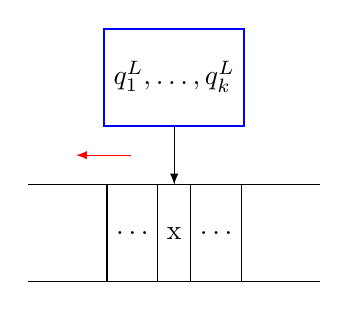
\begin{tikzpicture}[every node/.style={block},
        block/.style={minimum height=3.5em,outer sep=0pt,draw,rectangle,node distance=0pt}]
   \node (A) {\Mcell{x}{\cancelb}};
   \node (B) [left=of A] {$\ldots$};
   \node (D) [right=of A] {$\ldots$};
   \node (F) [above = 0.75cm of A,draw=blue,thick] {${q_1^L,\ldots,q_k^L}$};
   \draw[-latex] (F) -- (A);
   \draw[-latex,red] ($(F.west)!0.5!(B.east)$) -- ++(-7mm,0);
   \draw (B.north west) -- ++(-1cm,0) (B.south west) -- ++ (-1cm,0) 
                 (D.north east) -- ++(1cm,0) (D.south east) -- ++ (1cm,0);
\end{tikzpicture}
\end{aligned}
\]

    \item If the S-machine is in a left moving state, and the marker is $\cancelb$,
    then if will remain in a left moving set of states.
    In other words, if the cell is marked with $\cancelb$, the S-machine is guaranteed to move left, and
    leave the marker as $\cancelb$.  

\[
\begin{aligned}
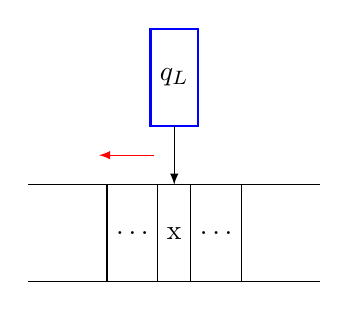
\begin{tikzpicture}[every node/.style={block},
        block/.style={minimum height=3.5em,outer sep=0pt,draw,rectangle,node distance=0pt}]
   \node (A) {\Mcell{x}{\cancelb}};
   \node (B) [left=of A] {$\ldots$};
   \node (D) [right=of A] {$\ldots$};
   \node (F) [above = 0.75cm of A,draw=blue,thick] {$q_L$};
   \draw[-latex] (F) -- (A);
   \draw[-latex,red] ($(F.west)!0.5!(B.east)$) -- ++(-7mm,0);
   \draw (B.north west) -- ++(-1cm,0) (B.south west) -- ++ (-1cm,0) 
                 (D.north east) -- ++(1cm,0) (D.south east) -- ++ (1cm,0);
\end{tikzpicture}
\end{aligned}
\quad \longrightarrow \quad
\begin{aligned}
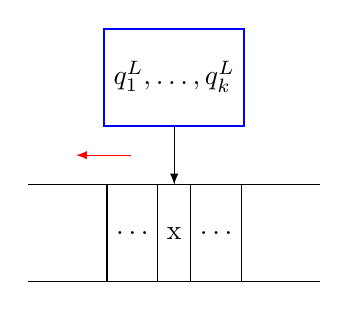
\begin{tikzpicture}[every node/.style={block},
        block/.style={minimum height=3.5em,outer sep=0pt,draw,rectangle,node distance=0pt}]
   \node (A) {\Mcell{x}{\cancelb}};
   \node (B) [left=of A] {$\ldots$};
   \node (D) [right=of A] {$\ldots$};
   \node (F) [above = 0.75cm of A,draw=blue,thick] {${q_1^L,\ldots,q_k^L}$};
   \draw[-latex] (F) -- (A);
   \draw[-latex,red] ($(F.west)!0.5!(B.east)$) -- ++(-7mm,0);
   \draw (B.north west) -- ++(-1cm,0) (B.south west) -- ++ (-1cm,0) 
                 (D.north east) -- ++(1cm,0) (D.south east) -- ++ (1cm,0);
\end{tikzpicture}
\end{aligned}
\]


    \item If the S-machine is in a left moving state, and it encounters $<\cancelc, \cancelc>$,
    it will enter a right moving state, and leave the $\cancelc$ marker in place.

\[
\begin{aligned}
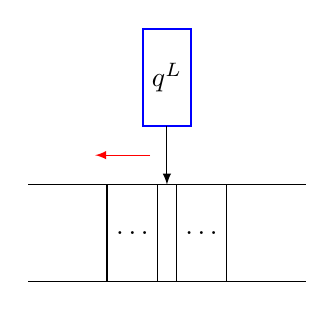
\begin{tikzpicture}[every node/.style={block},
        block/.style={minimum height=3.5em,outer sep=0pt,draw,rectangle,node distance=0pt}]
   \node (A) {\Mcell{\cancelc}{\cancelc}};
   \node (B) [left=of A] {$\ldots$};
   \node (D) [right=of A] {$\ldots$};
   \node (F) [above = 0.75cm of A,draw=blue,thick] {$q^L$};
   \draw[-latex] (F) -- (A);
   \draw[-latex,red] ($(F.west)!0.5!(B.east)$) -- ++(-7mm,0);
   \draw (B.north west) -- ++(-1cm,0) (B.south west) -- ++ (-1cm,0) 
                 (D.north east) -- ++(1cm,0) (D.south east) -- ++ (1cm,0);
\end{tikzpicture}
\end{aligned}
\quad \longrightarrow \quad
\begin{aligned}
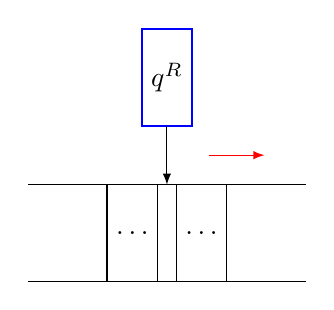
\begin{tikzpicture}[every node/.style={block},
        block/.style={minimum height=3.5em,outer sep=0pt,draw,rectangle,node distance=0pt}]
   \node (A) {\Mcell{\cancelc}{\cancelc}};
   \node (B) [left=of A] {$\ldots$};
   \node (D) [right=of A] {$\ldots$};
   \node (F) [above = 0.75cm of A,draw=blue,thick] {$q^R$};
   \draw[-latex] (F) -- (A);
   \draw[-latex,red] ($(F.east)!0.5!(D.east)$) -- ++(7mm,0);
   \draw (B.north west) -- ++(-1cm,0) (B.south west) -- ++ (-1cm,0) 
                 (D.north east) -- ++(1cm,0) (D.south east) -- ++ (1cm,0);
\end{tikzpicture}
\end{aligned}
\]


    \item If the S-machine is in a right moving state, and the marker is $\cancelb$, 
    it will remain in a right moving set of states.

\[
\begin{aligned}
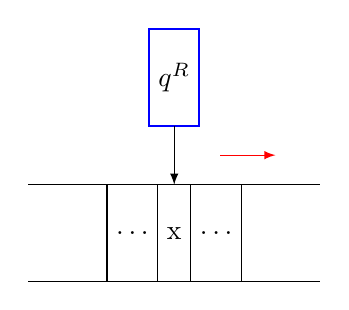
\begin{tikzpicture}[every node/.style={block},
        block/.style={minimum height=3.5em,outer sep=0pt,draw,rectangle,node distance=0pt}]
   \node (A) {\Mcell{x}{\cancelb}};
   \node (B) [left=of A] {$\ldots$};
   \node (D) [right=of A] {$\ldots$};
   \node (F) [above = 0.75cm of A,draw=blue,thick] {$q^R$};
   \draw[-latex] (F) -- (A);
   \draw[-latex,red] ($(F.east)!0.5!(D.east)$) -- ++(7mm,0);
   \draw (B.north west) -- ++(-1cm,0) (B.south west) -- ++ (-1cm,0) 
                 (D.north east) -- ++(1cm,0) (D.south east) -- ++ (1cm,0);
\end{tikzpicture}
\end{aligned}
\quad \longrightarrow \quad
\begin{aligned}
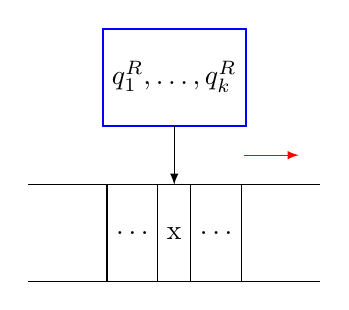
\begin{tikzpicture}[every node/.style={block},
        block/.style={minimum height=3.5em,outer sep=0pt,draw,rectangle,node distance=0pt}]
   \node (A) {\Mcell{x}{\cancelb}};
   \node (B) [left=of A] {$\ldots$};
   \node (D) [right=of A] {$\ldots$};
   \node (F) [above = 0.75cm of A,draw=blue,thick] {${q_1^R,\ldots,q_k^R}$};
   \draw[-latex] (F) -- (A);
   \draw[-latex,red] ($(F.east)!0.5!(D.east)$) -- ++(7mm,0);
   \draw (B.north west) -- ++(-1cm,0) (B.south west) -- ++ (-1cm,0) 
                 (D.north east) -- ++(1cm,0) (D.south east) -- ++ (1cm,0);
\end{tikzpicture}
\end{aligned}
\]


    \item If the S-machine is in a right moving state, and the marker is $z$ (blank), then
    it will enter a state in $P^R$ and mark the cell as $\cancelb$.

\[
\begin{aligned}
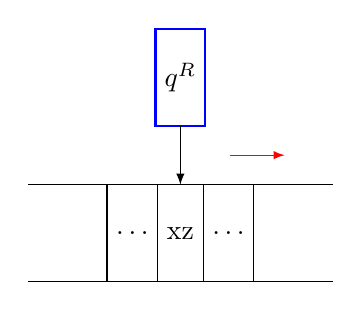
\begin{tikzpicture}[every node/.style={block},
        block/.style={minimum height=3.5em,outer sep=0pt,draw,rectangle,node distance=0pt}]
   \node (A) {\Mcell{x}{z}};
   \node (B) [left=of A] {$\ldots$};
   \node (D) [right=of A] {$\ldots$};
   \node (F) [above = 0.75cm of A,draw=blue,thick] {$q^R$};
   \draw[-latex] (F) -- (A);
   \draw[-latex,red] ($(F.east)!0.5!(D.east)$) -- ++(7mm,0);
   \draw (B.north west) -- ++(-1cm,0) (B.south west) -- ++ (-1cm,0) 
                 (D.north east) -- ++(1cm,0) (D.south east) -- ++ (1cm,0);
\end{tikzpicture}
\end{aligned}
\quad \longrightarrow \quad
\begin{aligned}
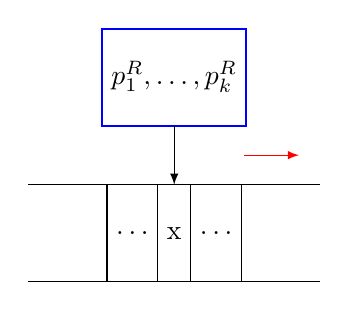
\begin{tikzpicture}[every node/.style={block},
        block/.style={minimum height=3.5em,outer sep=0pt,draw,rectangle,node distance=0pt}]
   \node (A) {\Mcell{x}{\cancelb}};
   \node (B) [left=of A] {$\ldots$};
   \node (D) [right=of A] {$\ldots$};
   \node (F) [above = 0.75cm of A,draw=blue,thick] {${p_1^R,\ldots,p_k^R}$};
   \draw[-latex] (F) -- (A);
   \draw[-latex,red] ($(F.east)!0.5!(D.east)$) -- ++(7mm,0);
   \draw (B.north west) -- ++(-1cm,0) (B.south west) -- ++ (-1cm,0) 
                 (D.north east) -- ++(1cm,0) (D.south east) -- ++ (1cm,0);
\end{tikzpicture}
\end{aligned}
\]


    \item If the s-machine is in state $p^R \ in P^R$, and the cell is marked with $\cancelb$,
    then it will mark the cell as $z$ (blank) and enter a left moving state.

 \[
\begin{aligned}
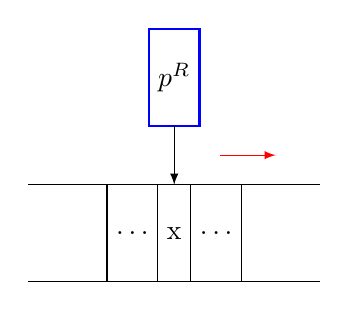
\begin{tikzpicture}[every node/.style={block},
        block/.style={minimum height=3.5em,outer sep=0pt,draw,rectangle,node distance=0pt}]
   \node (A) {\Mcell{x}{\cancelb}};
   \node (B) [left=of A] {$\ldots$};
   \node (D) [right=of A] {$\ldots$};
   \node (F) [above = 0.75cm of A,draw=blue,thick] {$p^R$};
   \draw[-latex] (F) -- (A);
   \draw[-latex,red] ($(F.east)!0.5!(D.east)$) -- ++(7mm,0);
   \draw (B.north west) -- ++(-1cm,0) (B.south west) -- ++ (-1cm,0) 
                 (D.north east) -- ++(1cm,0) (D.south east) -- ++ (1cm,0);
\end{tikzpicture}
\end{aligned}
\quad \longrightarrow \quad
\begin{aligned}
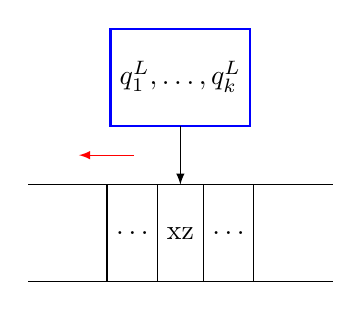
\begin{tikzpicture}[every node/.style={block},
        block/.style={minimum height=3.5em,outer sep=0pt,draw,rectangle,node distance=0pt}]
   \node (A) {\Mcell{x}{z}};
   \node (B) [left=of A] {$\ldots$};
   \node (D) [right=of A] {$\ldots$};
   \node (F) [above = 0.75cm of A,draw=blue,thick] {${q_1^L,\ldots,q_k^L}$};
   \draw[-latex] (F) -- (A);
   \draw[-latex,red] ($(F.west)!0.5!(B.east)$) -- ++(-7mm,0);
   \draw (B.north west) -- ++(-1cm,0) (B.south west) -- ++ (-1cm,0) 
                 (D.north east) -- ++(1cm,0) (D.south east) -- ++ (1cm,0);
\end{tikzpicture}
\end{aligned}
\]

\end{enumerate}

While stated above, it is important to realize that no matter how the machine operates,
all the set of states are synchronized with respect to their motion and the marker state of the cell.
So let us define first an augmented set of tape symbols that includes $\cancelb$:
\begin{equation*}
    \Sigma^+ = \Sigma \bigcup {\cancelb}
\end{equation*}
and let us also define a set of marker symbols 
\begin{equation*}
    Y = \{\cancelb, z\}
\end{equation*}

So it is more accurate to describe the contents of the tape cell as
\begin{equation*}
    \Gamma^* = \left\{
    \{<x_1,y>,\ldots,<x_k,y>\} | <x_i, y> \in \Sigma^+ \times Y \bigcup <\cancelc, \cancelc>
    \right\}
\end{equation*}

In words, this means each cell contains a 2-tuple, consisting of a set ${x_i}$ and a marker $y$, 
where
\begin{itemize}
    \item The set $x_i$ comes from either the input symbols or $\cancelb$.
    \item The marker $y$ is either $\cancelb$ or $z$.
    \item A special case symbol $<\cancelc, \cancelc>$, can appear, as can
    $<{\cancelc \ldots \cancelc}, \cancelc>$.
\end{itemize}

No other combination can appear.
It may be helpful to think of $\cancelb$ as a \verb|NULL| symbol.
\end{aside}


At any step $i$ of computation, $sc(i)$ will denote the index of the cell
scanned in~\ref{itm:scan} and $Ac(i)$ the set of
states at the end of~\ref{itm:state} above.
It follows that at step $i, i\geq 1$, the machine scans the
symbols of the cell $sc(i)$ in states $Ac(i-1)$.
In computing $Ac(i)$ from the symbols in cell
$sc(i)$ and the states $Ac(i-1)$, we use a choice function $\alpha$.
A particular choice function
$\alpha$ maps each state of $M$ to a subset of $\Gamma$.
Before defining this computation, we introduce
the notion of a product.

Let $A$ be the set of states and $B$ a set of tape symbols of $M$.
We introduce the following
operator $*$ called \emph{product}.
\begin{align*}
    A*B &= \left\{q|\exists x \in \Gamma, q_1 \in A, a_1 \in B \suchthat (q,x) \in \delta(q_1, a_1)\right\}\\
    B*A &= \left\{x|\exists q \in Q, q_1 \in A, a_1 \in B \suchthat (q_1,x) \in
    \delta(q_1, a_1)\right\}.
\end{align*}
\begin{error}
Typo?
Should be
\begin{align*}
    A*B &= \left\{q|\exists x \in \Gamma, q_1 \in A, a_1 \in B \suchthat (q,x) \in \delta(q_1, a_1)\right\}\\
    B*A &= \left\{x|\exists q \in Q, q_1 \in A, a_1 \in B \suchthat (q,x) \in
    \delta(q_1, a_1)\right\}.
\end{align*}
\end{error}
This $A*B$ is the set of all possible next states of $M$ and $B*A$ the set of all possible symbols
written in the scanned cell, when the machine state is a member of $A$ and the scanned cell a member
of $B$.

Henceforth, we shall refer to a set of states of $M$ as a \emph{stateset} and a set of tape symbols
of $M$ as a \emph{symbolset} respectively.
Statesets and symbolsets are closed under union.
Thus if $q_1, q_2$ are statesets, so is $q_1 + q_2$ and if $a_1, a_2$ are symbol subsets so is $a_1+a_2$.
The following lemma shows that distributive properties hold.
We use lower case symbols for statesets
and symbolsets.


\begin{lemma}\label{lem:distributive}
For any statesets $q, q_1, q_2$ and symbolsets $a, a_1, a_2$
\begin{align*}
    q*(a_1+a_2) &= q*a_1+q*a_2 \\
    (q_1 + q_2) * a &= q_1 * a + q_2 * a \\
    (a_1 + a_2) * q &= a_1 * q + a_2 * q \\
    a * (q_1 + q_2) &= a*q_1 + a*q_2
\end{align*}
\end{lemma}

\begin{proof}
    From the definition above,
    \begin{align*}
        p \in q * (a_1 + a_2) &\iff \exists p' \in q, x \in \Gamma, b \in a_1 + a_2 \suchthat (p,x) \in \delta(p', b) \\
        &\iff \exists p' \in q, x \in \Gamma, b \in a_1 \suchthat
        (p,x) \in \delta(p', b) \lor
        \exists p' \in q, x \in \Gamma, b \in a_2 \suchthat
        (p,x) \in \delta(p',b)\\
        &\iff p \in q * a_1 \lor p \in q * a_2 \\
        &\iff p \in q * a_1 + q * a_2
    \end{align*}
\end{proof}

\begin{aside}
    The original proof of Lemma~\ref{lem:distributive} is somewhat terse.
    However, the concept is fairly simple.
    From the definition of the product operator $*$, we have that
    $q * (a_1 + a_2)$ is the set of all states reachable from $q$, with
    a tape cell containing either $a_1$ or $a_2$.
    If $p$ is reachable from $q$ given a symbol from $a_1$ or $a_2$, then
    there must be an initial state $p' \in q$ such that we transition to
    $p$ with the symbol $b$ drawn from $a_1 + a_2$.
    We can then consider if the symbol $b$ comes from $a_1$ (in which case)
    $p \in q * a_1$, or if the symbol $b$ comes from $a_2$, in which case
    $p \in q * a_2$.
    If the symbol is common to both $a_1$ and $a_2$, the result is unaffected.
    As a result, we can claim that $p \in q*a_1 + q*a_2$.
\end{aside}

A stateset $q$ is \emph{left moving} if $q \subseteq Q^L$, \emph{right moving} if
$q \subseteq Q^R$ and halting if $q \cap H \neq \emptyset$.
\begin{error}
    Should this not be $q \subseteq Q^R \cup P^R$?
    The subset $P^R$ contains right moving states as well.
\end{error}
A symbolset $a$ is \emph{marked} if every tape symbol $x$ of $a$ contains the sweep marker.
The definitions of the instructions of $M$ show that a stateset of $M$ during any
computation is a left moving, right moving or a halting stateset.
The symbolset is either marked or unmarked.

Consider now the set of halting statesets $Q_H$.
If $M$ has been constructed to accept a recursive set $L$, then
for every input $w$ (encoded as defined subsequently), $M$ must halt
in an accepting or rejecting stateset.
Accordingly, we assume that $H = H_A \cup H_R$ where
$H_A$ is the set of accepting states and $H_R$ the set of
rejecting states.
$q \in Q_H$ is \emph{accepting} if $q \cap H_A \neq \emptyset$
and \emph{rejecting} if $q \cap H_A = \emptyset$.

We shall assume that there exist symbols $a_1, a_2 \in \Gamma$ such that
\[
    q \in H_A \implies \forall x \in \Gamma, \exists q' \in H_A \suchthat
    (q', a_1) \in \delta(q,x)
\]
and
\[
    q \in H_R \implies \forall x \in \Gamma, \exists q' \in H_R \suchthat
    (q', a_2) \in \delta(q,x).
\]
$a_1$ is therefore an accepting tapesymbol, and $a_2$ a rejecting
tapesymbol.  $H_A$ and $H_R$ would contain left moving and right moving states.

\begin{aside}
    The machine $M$ will write the symbol $a_1$ to the tape when it accepts the set $L$, and
    the machine $M$ will write the symbol $a_2$ to the tape when it rejects the set $L$.
\end{aside}

Let
\begin{align*}
    \Sigma_{A} &= \{a \subseteq \Gamma | a_1 \in a\} \\
    \Sigma_{R} &= \{a \subseteq \Gamma | a_2 \in a\} \\
    Q_A &= \{q \subseteq Q | q \cap H_A \neq \emptyset\} \\
    Q_R &= \{q \subseteq Q | q \cap H \neq \emptyset \land q \cap H_A \neq \emptyset \} \\
    \{Q\} &= \{q | q \subseteq Q^L \lor q \subseteq Q^R \}.
\end{align*}

\begin{error}
    Not sure why we don't need to consider $P^R$?
\end{error}

Then we have $Q_H = Q_A \cup Q_R, Q_A \cap Q_R = \emptyset$.
$\Sigma_A$ ($\Sigma_R$) is the set of accepting (rejecting) symbolsets,
$Q_A$ ($Q_R$) the set of accepting (rejecting) halt statesets and
${Q}$ the set of statesets of $M$.
We extend the product to sets of statesets.
Let $A, B$ be sets of
statesets and symbolsets respectively then,
\[
    A*B = \{q*a | q \in Q, a \in B\}
\]
and
\[
    B*A = \{a*q | q \in A, a \in B\}.
\]
Then, $\{Q\} * \Sigma_A \subseteq Q_A$, $\Sigma_A * \{Q\} \subseteq \Sigma_A$,
$\{Q\} * \Sigma_R \subseteq Q_R$ and $\Sigma_R * \{Q\} \subseteq \Sigma_R$.
Each $Q_A$ and $Q_R$ can be partitioned into leftmoving and rightmoving
parts, so that $Q_A = Q_A^L \cup Q_R^R$ and $Q_R = Q_R^L \cup Q_R^R$

\begin{error}
    I believe this is a typo.  Should be $Q_A = Q_A^L \cup Q_A^R$.
\end{error}

\begin{aside}
    Consider the first statement: $\{Q\} * \Sigma_A \subseteq Q_A$.
    In detail, this means that if we choose a stateset $q \in \{Q\}$,
    and a symbolset $a \in \Sigma_A$, then we know that by definition
    of $\Sigma_A$, that $a_1 \in a$ (i.e., at least one element of the
    symbolset is the special symbol $a_1$).
    From the definition of $a_1$, inclusion of this symbol in the
    symbolset guarantees that $M$ will halt and accept $L$.
    Similarly, if the symbolset under the tape head contains $a_1$,
    then at least one element of the output symbolset will also
    contain $a_1$.
\end{aside}

Suppose $w = a_1 a_2 \ldots a_n \in \Sigma^*$ be an imput string of length $n$.
The initial tape configuration of $M$ is the string of symbolsegs:
\[
    \left\{<\cancelc, \cancelc>\right\},
    \left\{<a_1,z>\right\},
    \left\{<a_2,\cancelb>\right\},
    \ldots
    \left\{<a_n,\cancelb>\right\}.
\]
The leftmost symbolset is assumed to be in the cell with index 0.
Cells with index $> n$ are assumed to contain $\{<\cancelb,\cancelb>\}$.
The initial stateset is $\{q_0\}$, and the cell scanned is 1.


\begin{aside}
%        |{q_0}|
%           |
%           v
%  | \c |  a_1  |  a_2  |  ...  |  a_n  |  \b  |  ....
%  | \c |   z   |   \b  |       |   \b  |  \b  |
%    A      B       C       D       E       F     G
%
    This is a diagram of $M$ in its initial state.
\begin{center}
\begin{tikzpicture}[every node/.style={block},
    block/.style={minimum height=3.5em,outer sep=0pt,draw,rectangle,node distance=0pt}]
    \node (A) {\Mcell{\cancelc}{\cancelc}};
    \node (A0) [below=of A, draw=none] {$0$};
    \node (B) [right=of A] {\Mcell{a_1}{z}};
    \node (B0) [below=of B, draw=none] {$1$};
    \node (C) [right=of B] {\Mcell{a_2}{\cancelb}};
    \node (C0) [below=of C, draw=none] {$2$};
    \node (D) [right=of C] {$\ldots$};
    \node (E) [right=of D] {\Mcell{a_n}{\cancelb}};
    \node (E0) [below=of E, draw=none] {$n$};
    \node (F) [right=of E] {\Mcell{\cancelb}{\cancelb}};
    \node (G) [right=of F] {$\ldots$};
    \node (F) [above = 0.75cm of B,draw=blue,thick] {$q_0$};
    \draw[-latex] (F) -- (B);
    \draw (A.north west) -- ++(-1cm,0) (A.south west) -- ++ (-1cm,0)
    (G.north east) -- ++(1cm,0) (G.south east) -- ++ (1cm,0);
\end{tikzpicture}
\end{center}
\end{aside}

From rule~\ref{itm:start}\footnote{Original says "rule 1".}
of $M$, the machine would rewrite the symbol set in cell $1$ and move left.
Step 1 of the computation of $M$ begins with $M$ scanning $\cell{0} = sc(1)$ in
stateset $Ac(0)$ where
\[
    Ac(0) = \{q_0\} * \{<a_1, z>\}
\]
and $\cellp{1}$ denotes the contents of $\cell{1}$ at the end of the initial step.
From rules~\ref{itm:start} of $M$, $Ac(0) \subseteq Q^L$ and $sc(i) = 0$.
The function $sc(i)$ defining the index of the scanned cell at step $i$ can
be obtained from the description of $M$.
In general
\[
    sc(1) = 0
\]
and for $i > 1$:
\begin{align*}
    sc(i+1) =
    \begin{cases}
        sc(i)+1 \,\mathrm{if}\,Ac(i) \subseteq Q^R \lor sc(i) = 0 \\
        sc(i)-1 \,\mathrm{if}\,Ac(i) \subseteq Q^L \land sc(i) > 1 \lor Ac(i) \subseteq P^R.
    \end{cases}
\end{align*}
If the scanned cell at step $i$ is to the right of cell $0$ and the machine moves
left at the end of step $i$ then the index of the scanned cell at step $i+1$
is one less than that at step $i$.
A left move at the end of step $i$ happens
if either $Ac(i) \subseteq Q^L$ or by rule~\ref{itm:turnaround} of $M$,
$Ac(i) \subseteq P^R$.
If $Ac(i) \subseteq Q^R$ or $sc(i) = 0$, the machine moves right at the end of the
$i$th step, so that the index of the scanned cell at step $i+1$ is obtained by
adding one to that at step $i$i.
A \emph{choice function} $\alpha : Q \mapsto 2^\Gamma$ maps each state of $M$ to
a subset of tape symbols.
Since there are only finitely many states and tape symbols, there are only
finitely many possible choice functions.

For a given initial configuration, $(Ac(0), sc(1))$, a computation of length $n$
of the S-machine $M$ is uniquely described by a sequence $\alpha_1,\alpha_2,\ldots,
\alpha_n$ of choice functions.
Symbolically,
\[
    (Ac(i), sc(i+1)) \, \xrightarrow[\alpha_{i+1}]{} \, (Ac(i+1), sc(i+2))
\]
for $0 \leq i < n$.

We have defined $Ac(1), sc(2)$ above.
Given $Ac(i), sc(i+1)$ and a choice function $\alpha_{i+1}$ we define
below $Ac(i+1)$ and cell $(sc(i+1))$ after the completion of the $(i+1)$st step.  Since $sc(i+1)$ and $Ac(i+1)$ are not
now known, $sc(i+2)$ can be computed.
We shall use the notion $\cellp{sc(i+1)}$ to denote the contents of $\cell{sc(i+1)}$
after the completion of the $(i+1)$st step.
$\cell{sc(i+1)}$ denotes the contents of $\cell{sc(i+1)}$ at the beginning of the $(i+1)$st step.




\section{Equivalence of statesets and symbol sets}\label{sec:two}
\section{The left context graph}\label{sec:three}
\section{Properties of $G_i$}\label{sec:four}
\section{Uniformity of $\bar{P}_2$}\label{sec:five}
\section{Appendix}\label{sec:appendix}
\subsection{Proofs for Lemma~\ref{lem:distributive}}\label{ssec:distributive_proofs}

The proofs of the various parts of Lemma~\ref{lem:distributive} were left out of the original
paper as they are straightforward.
In the interest of completion, we include those proofs in this appendix subsection.
First, we prove that for any statesets $q, q_1, q_2$ and symbolsets $a, a_1, a_2$
\begin{align*}
    (q_1 + q_2) * a &= q_1 * a + q_2 * a \\
\end{align*}

\begin{proof}
    \begin{align*}
        p \in (q_1 + q_2) * a & \iff \exists p' \in (q_1+q_2), x \in \Gamma \suchthat (p,x) \in \delta(p', a) \\
        & \iff p' \in q_1, x \in \Gamma \suchthat (p,x) \in \delta(p', a) \lor
               p' \in q_2, x \in \Gamma \suchthat (p,x) \in \delta(p', a) \\
        & \iff p \in q_1 * a \lor p \in q_2 * a \\
        & \iff p \in q_1 * a + q_2 * a
    \end{align*}
\end{proof}

Next, we prove
\begin{align*}
    (a_1 + a_2) * q &= a_1 * q + a_2 * q.
\end{align*}

\begin{proof}
    \begin{align*}
        b \in (a_1 + a_2) * q & \iff \exists p' \in Q, p \in q, x \in (a_1 + a_2) \suchthat (p',b) \in \delta(p,x) \\
        & \iff \exists p' \in Q, p \in Q, x \in a_1 \suchthat (p', b) \in \delta(p,x) \lor
         \exists p' \in Q, p \in Q, x \in a_2 \suchthat (p', b) \in \delta(p,x) \\
        & \iff b \in a_1 * q \lor b \in a_2 * q \\
        & \iff b \in a_1 * q + a_2 * q
    \end{align*}
\end{proof}

Finally, we prove
\begin{align*}
    a * (q_1 + q_2) &= a*q_1 + a*q_2
\end{align*}

\begin{proof}
    \begin{align*}
        b \in a * (q_1 + q_2) & \iff \exists p' \in Q, p \in (q_1 + q_2), x \in a \suchthat (p', b) \in \delta(p, x) \\
        & \iff \exists p' \in Q, p \in q_1, x \in q \suchthat (p', b) \in \delta(p, x) \lor
        \exists p' \in Q, p \in q_2, x \in q \suchthat (p', b) \in \delta(p, x) \\
        & \iff b \in a * q_1 \lor b \in a * q_2 \\
        & \iff b \in a * q_1 + a * q_2
    \end{align*}
\end{proof}
\end{document}